\clearpage
\section{Έλεγχοι με επαγωγικές διαδικασίες και η στατιστική ερμηνεία τους (Β \& Γ)}

\subsection{Έλεγχος ανεξαρτησίας \lat{$X^2$}}
Με βάση τα παραπάνω στοιχεία τα οποία  είναι αποτέλεσμα του ερωτήματος Α απορρέουν μερικά ερωτήματα τα οποία μπορούν να ελεγχθούν με συγκεκριμένες επαγωγικές διαδικασίες.

Αρχικά, θα ήταν σκόπιμο να ελέγξουμε την ανεξαρτησία ορισμένων μεταβλητών οι οποίες θεωρούνται χαρακτηριστικές. \textbf{Η σχέση ανάμεσα στην μεταβλητή "Πρώτο καρδιακό επεισόδιο" και την "Οικογενειακό ιστορικό" θα ήταν ενδιαφέρον να ερευνηθεί για τυχόν ύπαρξη σχέσης ανάμεσα τους.}

Με την εφαρμογή του ελέγχου ανεξαρτησίας \lat{$X^2$} παίρνουμε τις παρακάτω πληροφορίες σε μορφή πινάκων.

\begin{figure}[h]
    \centering
    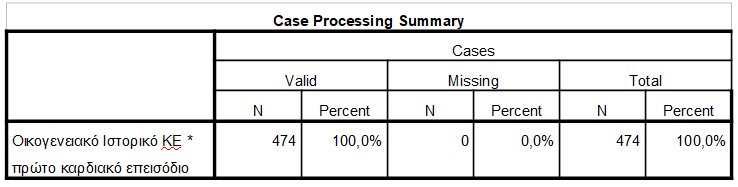
\includegraphics[width=0.8\textwidth]{images/100.PNG}
\end{figure}

Στον πίνακα \textbf{Case Processing Summary},όπως και παραπάνω με τον πίνακα \textbf{Statistics} μπορούμε να πάρουμε πληροφορίες για τυχόν cases που δεν συμπεριλήφθησαν από την στήλη Missing. Όπως είναι εμφανές, από ένα σύνολο 474 cases, όλες λήφθησαν υπόψη.

\begin{figure}[h]
    \centering
    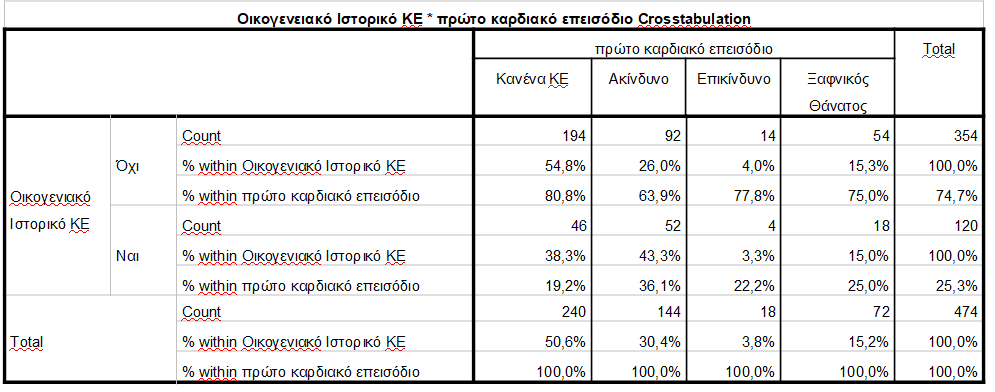
\includegraphics[width=\textwidth]{images/101.PNG}
\end{figure}

Από τον πίνακα συνάφειας παρατηρούμε τα εξής: 
\begin{itemize}
    \item Όσοι δεν είχαν κανένα καρδιακό επεισόδιο χωρίς οικογενειακό ιστορικό (80,8\%) εμφανίζουν μεγαλύτερο ποσοστό σε σχέση με όσους είχαν οικογενειακό ιστορικό (19,2\%).
    \item Όσοι υπέστησαν ακίνδυνο καρδιακό επεισόδιο χωρίς οικογενειακό ιστορικό (63,9\%) είναι σχεδόν διπλάσιοι σε ποσοστό σε σχέση με αυτούς που είχαν οικογενειακό ιστορικό (36,1\%). 
    \item Επιπλέον παρατηρείται ότι το ποσοστό εμφάνισης καρδιακού επεισοδίου (από κανένα σε ακίνδυνο καρδιακό) αυξάνεται σχεδόν στο διπλάσιο για όσους έχουν οικογενειακό ιστορικό.
\end{itemize}

\begin{figure}[h]
    \centering
    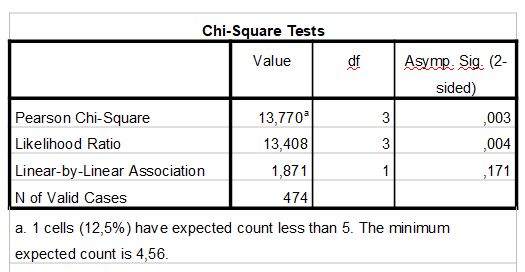
\includegraphics[width=0.8\textwidth]{images/102.PNG}
\end{figure}

Στον πίνακα \lat{Chi-Square Tests} παρατηρούμε ότι \lat{$X^2=13,77$} και p=0,003. Δηλαδή, πρόκειται για ένα στατιστικά σημαντικό τεστ. Επιπλέον, δεδομένου ότι το \lat{$p<0,05$},  μπορούμε να συμπεράνουμε ότι οι μεταβλητές  "Οικογενειακό Ιστορικό" και "Πρώτο Καρδιακό Επεισόδιο" συσχετίζονται η μία με την άλλη. Κατά συνέπεια, απορρίπτουμε την μηδενική υπόθεση καθώς \textbf{υπάρχει εξάρτηση ανάμεσα στις δύο αυτές μεταβλητές}.

Στην συνέχεια θα μελετήσουμε την σχέση εξάρτησης ανάμεσα στις μεταβλητές "Πρώτο Καρδιακό Επεισόδιο" και "Επιβίωση μετά από 10 χρόνια". 

\begin{figure}[h]
    \centering
    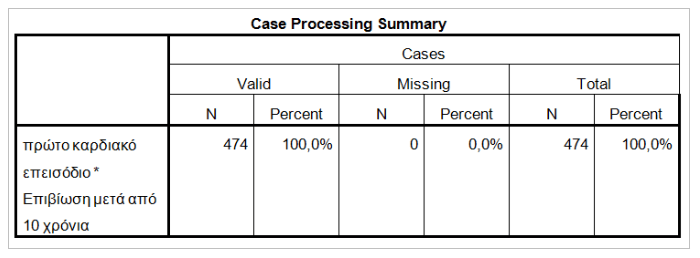
\includegraphics[width=0.8\textwidth]{images/103.PNG}
\end{figure}

Στον πίνακα \textbf{Case Processing Summary}, όπως και προηγουμένως παρατηρούμε ότι όλες οι τιμές λήφθησαν υπόψιν.
\clearpage

\begin{figure}[h]
    \centering
    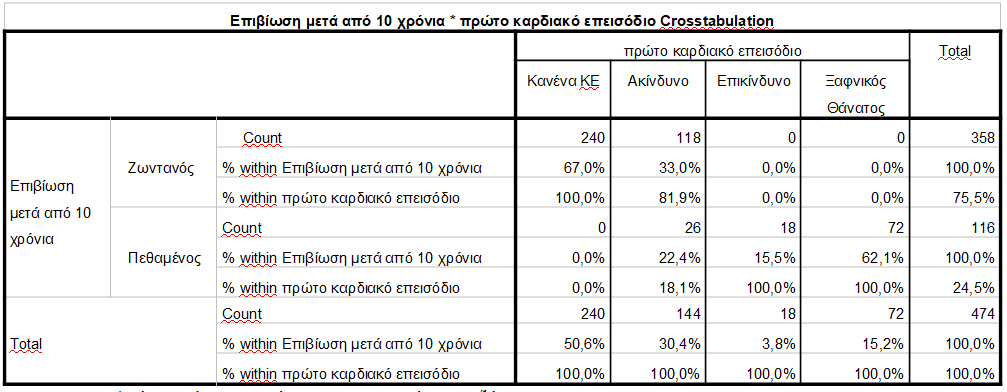
\includegraphics[width=\textwidth]{images/104.PNG}
\end{figure}

Από τον πίνακα συνάφειας παρατηρούμε τα εξής:
\begin{itemize}
    \item Για όσους δεν υπέστησαν κανένα καρδιακό επεισόδιο η θνησιμότητα είναι μηδενική μετά από 10 χρόνια. 
    \item Σε όσους υπέστησαν ακίνδυνο πρώτο καρδιακό επεισόδιο το μεγαλύτερο ποσοστό παρέμεινε ζωντανό μετά από 10 χρόνια (81,9\%) σε σχέση με όσους απεβίωσαν (18,1\%).
    \item Όσον αφορά τις υποκατηγορίες επικίνδυνο και ξαφνικός θάνατος τα αποτελέσματα που προέκυψαν είναι απολύτως λογικά, καθώς η θνησιμότητα φτάνει σε ποσοστό 100\%.
\end{itemize}

\begin{figure}[h]
    \centering
    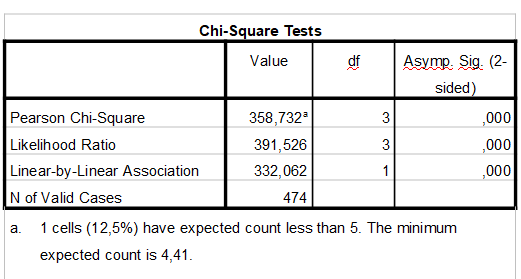
\includegraphics[width=0.8\textwidth]{images/105.PNG}
\end{figure}

Στον πίνακα Chi-Square Tests παρατηρούμε ότι \lat{$X^2=358,73$} και p=0,0001. Δηλαδή, πρόκειται για ένα στατιστικά σημαντικό τεστ. Επιπλέον, δεδομένου ότι το \lat{$p<0,05$}, μπορούμε να συμπεράνουμε ότι οι μεταβλητές  "Πρώτο Καρδιακό Επεισόδιο" και "Επιβίωση μετά από 10 χρόνια" συσχετίζονται η μία με την άλλη. Κατά συνέπεια, απορρίπτουμε την μηδενική υπόθεση καθώς \textbf{υπάρχει εξάρτηση ανάμεσα στις δύο αυτές μεταβλητές}.

\clearpage
Στην συνέχεια θα μελετήσουμε την σχέση εξάρτησης ανάμεσα στις μεταβλητές "Οικογενειακό Ιστορικό ΚΕ" και "Επιβίωση μετά από 10 χρόνια".

\begin{figure}[h]
    \centering
    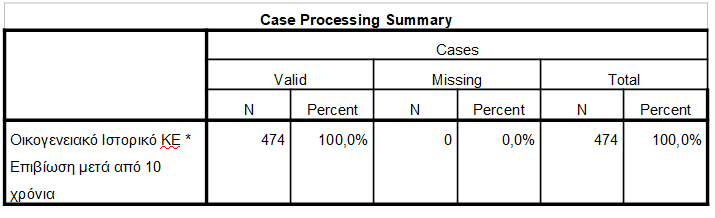
\includegraphics[width=0.8\textwidth]{images/106.PNG}
\end{figure}

Στον πίνακα \textbf{Case Processing Summary},όπως και προηγουμένως παρατηρούμε ότι όλες οι τιμές λήφθησαν υπόψη. 

\begin{figure}[h]
    \centering
    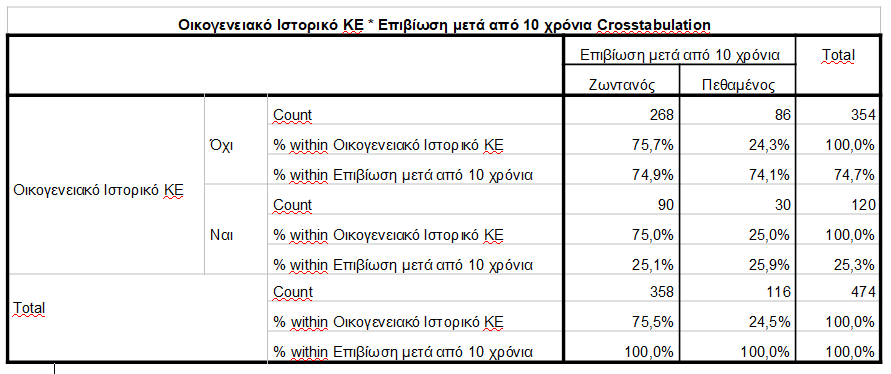
\includegraphics[width=\textwidth]{images/107.PNG}
\end{figure}

Από τον πίνακα συνάφειας παρατηρούμε τα εξής:
\begin{itemize}
    \item Το ποσοστό των ατόμων που επιβίωσαν μετά από 10 χρόνια χωρίς να έχουν οικογενειακό ιστορικό ΚΕ είναι περισσότεροι σε σχέση με αυτούς που έχουν.
    \item Αυτό που αξίζει να τονιστεί είναι πως το ποσοστό των ατόμων που απεβίωσαν μετά από 10 χρόνια είναι μεγαλύτερο για όσους δεν έχουν οικογενειακό ιστορικό ΚΕ (74,1\%) σε σχέση με όσους έχουν (25,9\%).
\end{itemize}

\clearpage

\begin{figure}[h]
    \centering
    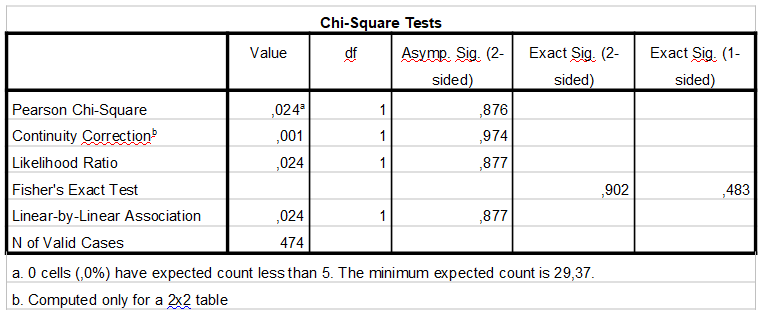
\includegraphics[width=0.8\textwidth]{images/108.PNG}
\end{figure}

Στον πίνακα \lat{Chi-Square Tests} παρατηρούμε ότι \lat{$X^2=0,024$} και p=0,876. Είναι προφανές ότι δεν υπάρχει ιδιαίτερη συσχέτιση ανάμεσα στις δύο μεταβλητές. Συγκεκριμένα, από την τιμή του p-value η οποία είναι μεγαλύτερη του 5\% μπορούμε να πούμε ότι οι δύο αυτές μεταβλητές \textbf{είναι ανεξάρτητες μεταξύ τους}.

Αξίζει να σημειωθεί πως το ποσοστό που υπάρχει στην παρένθεση της υποσημείωσης σε όλους τους πίνακες \lat{$\textbf{X}^\textbf{2}$} αναφέρεται στο ποσοστό των αναμενόμενων συχνοτήτων που είναι μικρότερες από 5 και δεν ξεπερνάει το 20\%.

\subsection{Έλεγχοι διαφορών ως προς μεταβλητές \lat{nominal}}

\subsubsection{Έλεγχος κανονικότητας}

Ξεκινώντας με τις μεταβλητές "Αριθμός Τσιγάρων ανά Ημέρα" και "Επιβίωση μετά από 10 χρόνια". Μέσω του ελέγχου ως προς την κανονική κατανομή με το \lat{Kolmogorov-Smirnov} και \lat{Shapiro-Wilk} παίρνουμε τους παρακάτω πίνακες και διαγράμματα. 

\begin{figure}[h]
    \centering
    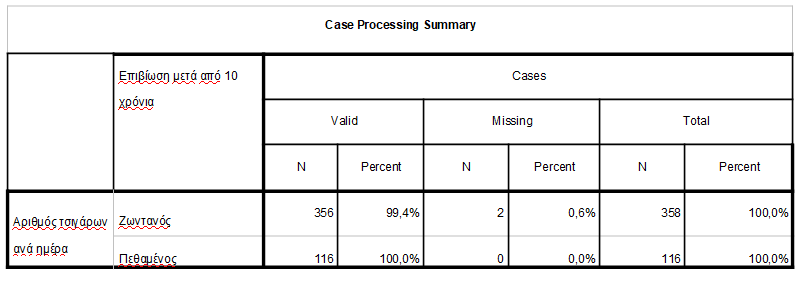
\includegraphics[width=0.8\textwidth]{images/109.PNG}
\end{figure}

Ο πίνακας \textbf{Case Processing Summary}, όπως και προηγουμένως μας δίνει πληροφορίες για το πόσα από τα cases που υπήρχαν αρχικά στο αρχείο μας, λήφθηκαν υπόψιν.

\clearpage

\begin{figure}[h]
    \centering
    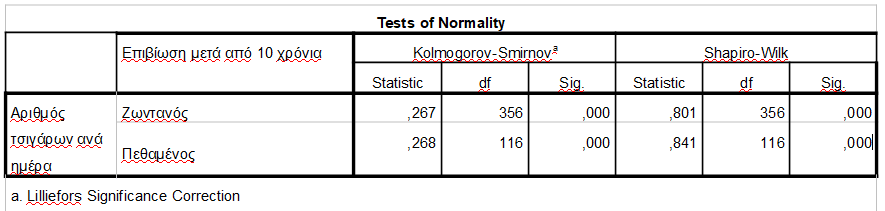
\includegraphics[width=0.8\textwidth]{images/110.PNG}
\end{figure}

Από τον πίνακα \lat{Tests of Normality} μπορούμε να πάρουμε αποτελέσματα από δύο τεστ κανονικότητας, τα \lat{Kolmogorov-Smirnov} και \lat{Shapiro-Wilk}.Το δεύτερο χρησιμοποιείται κυρίως για μικρά δείγματα ενώ το πρώτο δίνει καλά  αποτελέσματα και για μεγάλα. Στην περίπτωση μας έχουμε δείγμα από 474 ασθενείς οπότε θα χρησιμοποιήσουμε το πρώτο. Παρατηρώντας τον πίνακα βλέπουμε ότι το p-value και στις δύο περιπτώσεις είναι κατά πολύ μικρότερο του 5\%. Συνεπώς, τα δεδομένα μας αποκλίνουν από την κανονικότητα.

Αποτελέσματα για την κανονικότητα μπορούμε να πάρουμε και γραφικά μέσω των \lat{Q-Q plots}. Όπως βλέπουμε και στα δύο διαγράμματα, τα δεδομένα μας έχουν την τάση να απομακρυνθούν από την διαγώνιο. Κατά συνέπεια, τα διαγράμματα όπως ήταν αναμενόμενο συμφωνούν με τον πίνακα.


\begin{figure}[h]
    \centering
    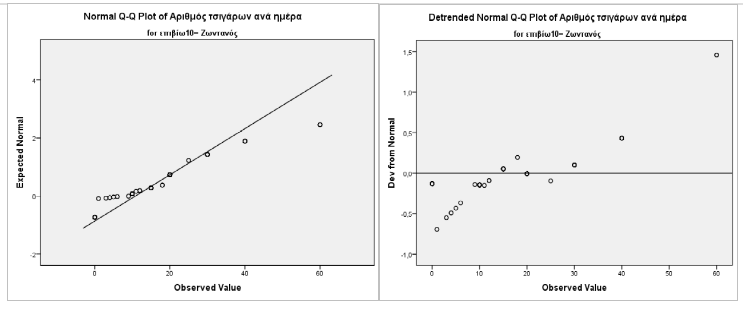
\includegraphics[width=0.8\textwidth]{images/111.PNG}
\end{figure}

\begin{figure}[h]
    \centering
    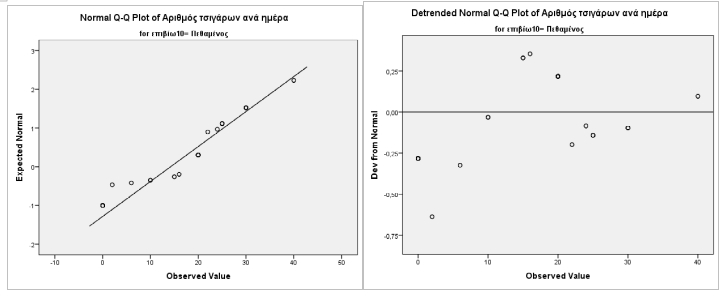
\includegraphics[width=0.8\textwidth]{images/112.PNG}
\end{figure}

\clearpage

\begin{figure}[h]
    \centering
    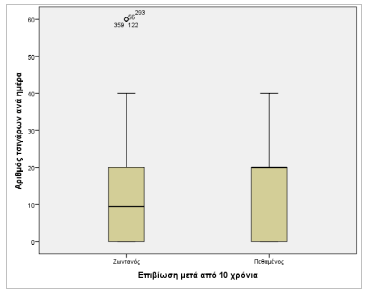
\includegraphics[width=0.8\textwidth]{images/113.PNG}
\end{figure}

Παρατηρούμε ότι από τον πίνακα \textbf{\lat{Test Statistics}} υπάρχει σημαντική διαφορά ανάμεσα στις μέσες τιμές των μεταβλητών Επιβίωση μετά από 10 χρόνια και Αριθμού τσιγάρων σύμφωνα με το \lat{Mann-Whitney}. Αυτό προκύπτει από το γεγονός ότι το p-value είναι <5\%. Συμπεραίνουμε  ότι τα άτομα που δεν επιβίωσαν είχαν την τάση να καπνίζουν περισσότερα τσιγάρα.

\vspace{2cm}

 \begin{figure}[h]
     \centering
     \begin{subfigure}{0.8\textwidth}
     \centering
         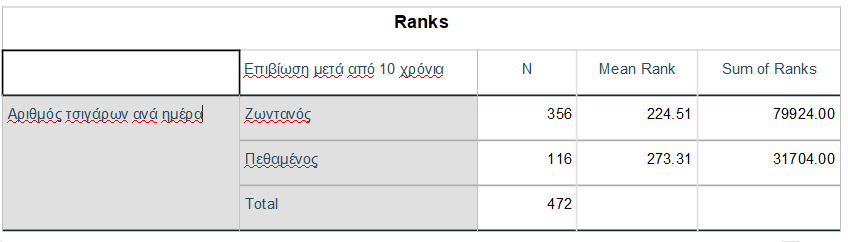
\includegraphics[width=\textwidth]{images/114.PNG}
              \end{subfigure}
              \end{figure}
     
     \clearpage
     
     \begin{figure}[ht]\ContinuedFloat
     \centering
     \begin{subfigure}{0.8\textwidth}
     \centering
         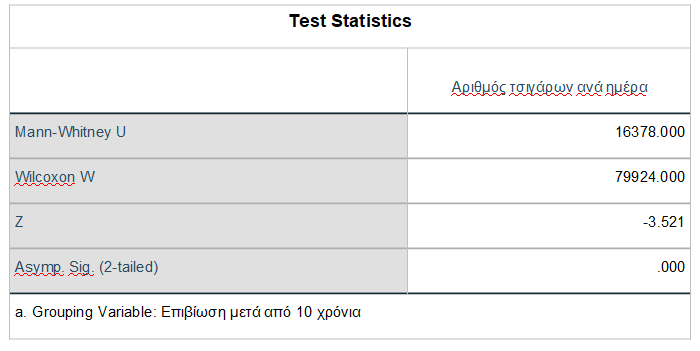
\includegraphics[width=\textwidth]{images/115.PNG}
             \end{subfigure}
      
\end{figure}

Ο πίνακας \textbf{\lat{Case Processing Summary}}  μας δίνει πληροφορίες για το πόσα από τα cases που υπήρχαν αρχικά στο αρχείο μας, λήφθηκαν υπόψιν.

\begin{figure}[h]
    \centering
    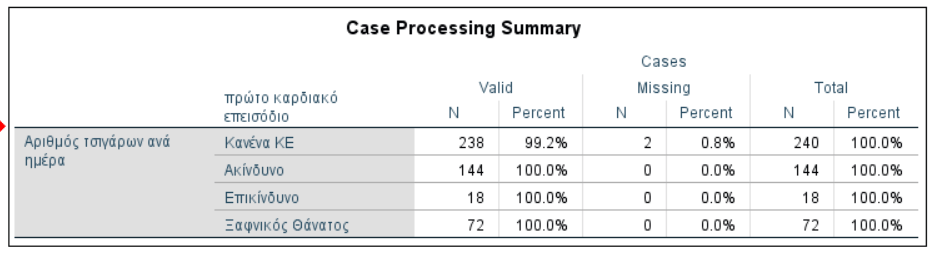
\includegraphics[width=\textwidth]{images/200.PNG}
\end{figure}

\vspace{1cm}
Από τον πίνακα Tests of Normality μπορούμε να πάρουμε αποτελέσματα από δύο τεστ κανονικότητας, τα Kolmogorov-Smirnov και Shapiro-Wilk. Παρατηρώντας τον πίνακα βλέπουμε ότι το p-value και στις δύο περιπτώσεις είναι κατά πολύ μικρότερο του 5\%.  Άρα οι μεταβλητές μας δεν ακολουθούν κανονική κατανομή.

Όσο αναφορά την κατηγορία “Επικίνδυνο” έχουμε λίγες μετρήσεις και αρκετές ακραίες τιμές. Όμως η αφαίρεση τους αφήνει το δείγμα με 12 μόνο μετρήσεις με αποτέλεσμα τα \lat{tests} κανονικότητας να μην δίνουν αποτελέσματα. Αξίζει να αναφέρουμε ότι τα δεδομένα για αυτήν την κατηγορία προφανώς δεν είναι αρκετά αλλά από ερευνητική σκοπιά κρίναμε αναγκαίο να μελετηθούν οι επιπτώσεις του τσιγάρου όσο αναφορά το “πρώτο καρδιακό επεισόδιο”. Επιπλέον οι μη παραμετρικοί έλεγχοι  μπορούν να εφαρμοστούν σε περιπτώσεις πολύ μικρών δειγμάτων.

\clearpage

\begin{figure}[h]
    \centering
    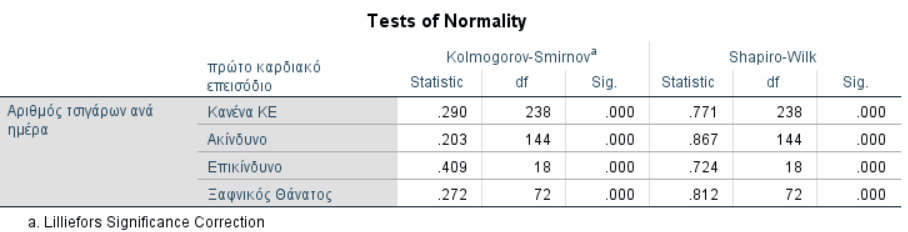
\includegraphics[width=\textwidth]{images/201.PNG}
\end{figure}

\vspace{1cm}

\begin{figure}[h]
 \centering

     \begin{subfigure}{0.8\textwidth}
     \centering
         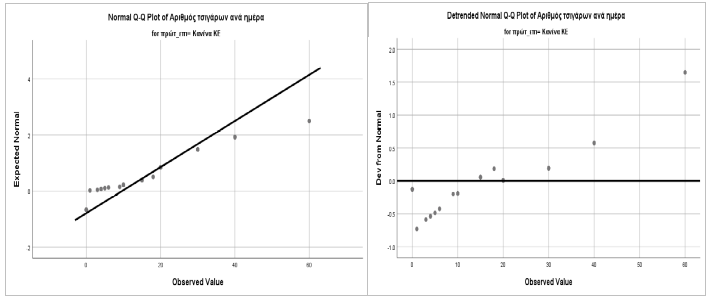
\includegraphics[width=\textwidth]{images/300.PNG}
                      \end{subfigure}
     \vspace{1cm}
     
     \begin{subfigure}{0.8\textwidth}
     \centering
         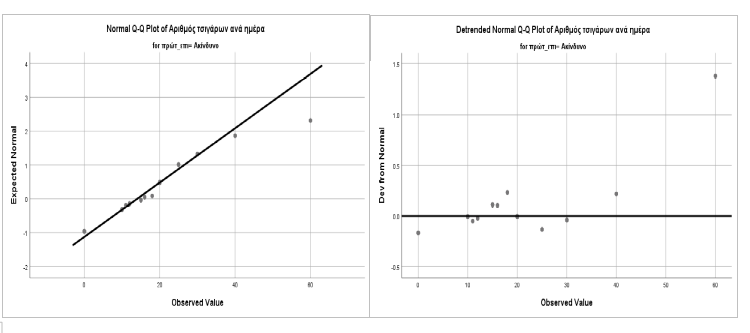
\includegraphics[width=\textwidth]{images/301.PNG}
             \end{subfigure}
\end{figure}

\clearpage

\begin{figure}
 \centering

     \begin{subfigure}{0.8\textwidth}
     \centering
         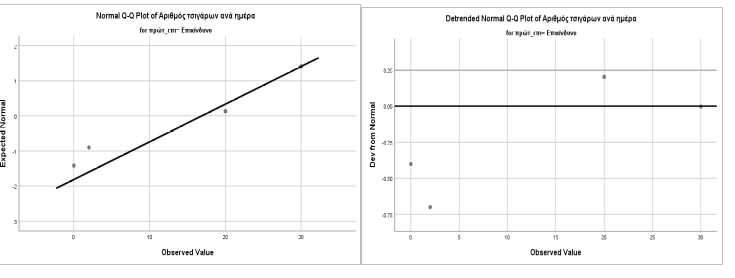
\includegraphics[width=\textwidth]{images/302.PNG}
                      \end{subfigure}
                      
     \vspace{2cm}
     
     \begin{subfigure}{0.8\textwidth}
     \centering
         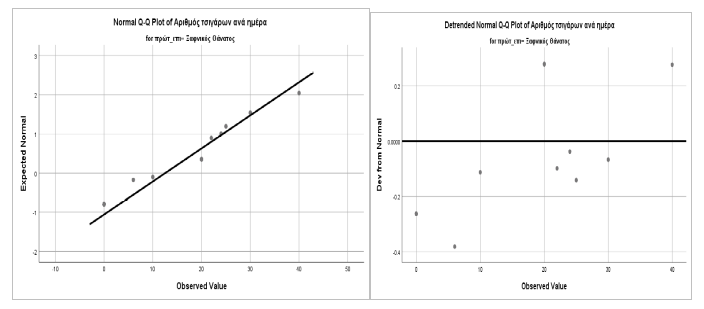
\includegraphics[width=\textwidth]{images/303.PNG}
             \end{subfigure}
\end{figure}

\clearpage

\begin{figure}[ht]
    \centering
    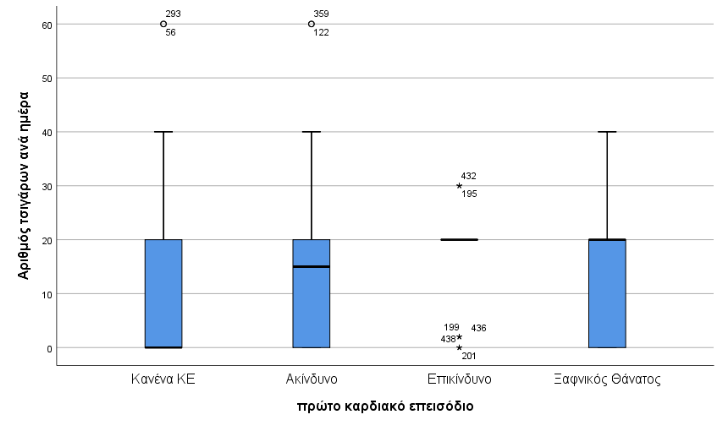
\includegraphics[width=\textwidth]{images/304.png}
\end{figure}

Παρατηρούμε ότι από τον πίνακα \textbf{\lat{Test Statistics}} υπάρχει σημαντική διαφορά ανάμεσα στις μέσες τιμές των μεταβλητών "Πρώτο καρδιακό επεισόδιο" και τον "Αριθμό τσιγάρων". Αυτό προκύπτει από το γεγονός ότι το p-value είναι <5\%.  Συμπεραίνουμε ότι ο αριθμός τσιγάρων φαίνεται να επηρεάζει την επικινδυνότητα του πρώτου καρδιακού επεισοδίου.

\begin{figure}[h]
    \centering
    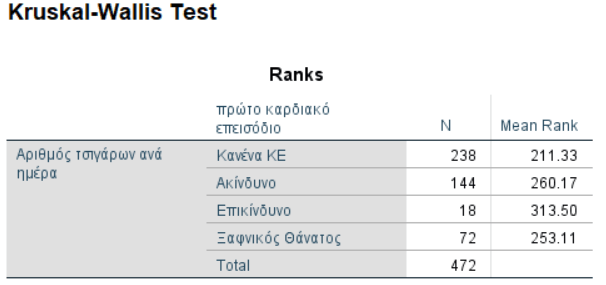
\includegraphics[width=0.9\textwidth]{images/202.PNG}
\end{figure}

\clearpage

\begin{figure}[ht]
    \centering
    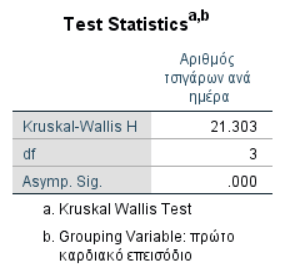
\includegraphics[width=0.4\textwidth]{images/203.PNG}
\end{figure}

Εφόσον το \lat{Kruskal-Wallis} δείχνει ότι υπάρχουν σημαντικές διαφορές στις μέσες τιμές, θα πραγματοποιήσουμε τον έλεγχο \lat{Mann-Whitney}, ώστε να εντοπιστούν οι κατηγορίες στις οποίες εμφανίζονται οι διαφορές. 

\vspace{1cm}

\begin{figure}[ht]
    \centering
    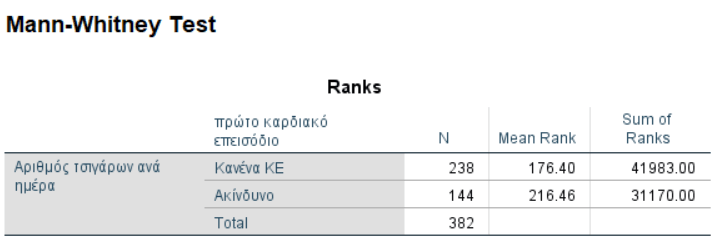
\includegraphics[width=0.8\textwidth]{images/204.PNG}
\end{figure}

\vspace{1cm}
Παρατηρούμε ότι από τον πίνακα \textbf{\lat{Test Statistics}} υπάρχει σημαντική διαφορά ανάμεσα στις μέσες τιμές των μεταβλητών "Κανένα ΚΕ" και "Ακίνδυνο" σε σχέση με τον "Αριθμό τσιγάρων". Αυτό προκύπτει από το γεγονός ότι το p-value είναι <5\%. Συμπεραίνουμε  ότι τα άτομα που είναι στην κατηγορία "Κανένα ΚΕ"  είχαν την τάση να καπνίζουν λιγότερα τσιγάρα σε σχέση με αυτά της κατηγορίας "Ακίνδυνο".

\clearpage

\begin{figure}[ht]
    \centering
    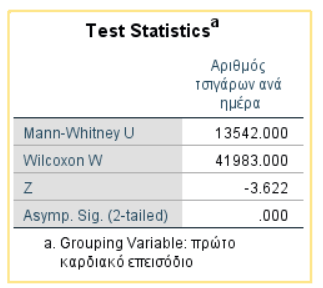
\includegraphics[width=0.4\textwidth]{images/205.PNG}
\end{figure}

Για τις διαφορές “Κανένα ΚΕ” και “Επικίνδυνο” φαίνεται και εδώ στατιστικά σημαντική διαφορά στις μέσες τιμές σε σχέση με τον “Αριθμό τσιγάρων”. Αυτό προκύπτει από το γεγονός ότι το p-value είναι <5\%. Φαίνεται να καπνίζουν λιγότερο τα άτομα στην κατηγορία “Κανένα ΚΕ” σε σχέση με αυτούς στην κατηγορία “Επικίνδυνο”.

\vspace{1cm}

\begin{figure}[h]
    \centering
    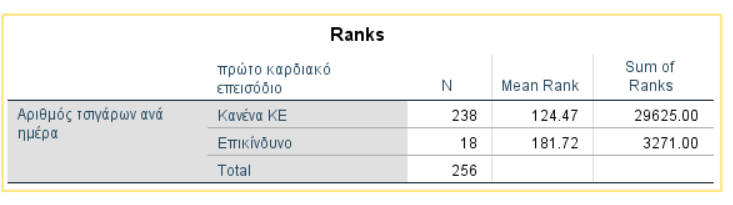
\includegraphics[width=0.8\textwidth]{images/206.PNG}
\end{figure}

\vspace{1cm}

\begin{figure}[h]
    \centering
    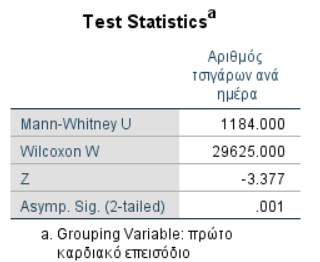
\includegraphics[width=0.4\textwidth]{images/207.PNG}
\end{figure}

\clearpage

Για τις διαφορές “Κανένα ΚΕ” και “Ξαφνικός θάνατος” φαίνεται και εδώ στατιστικά σημαντική διαφορά στις μέσες τιμές σε σχέση με τον “Αριθμό τσιγάρων”. Αυτό προκύπτει από το γεγονός ότι το p-value είναι <5\%. Φαίνεται να καπνίζουν λιγότερο τα άτομα στην κατηγορία “Κανένα ΚΕ” σε σχέση με αυτούς στην κατηγορία “Ξαφνικός θάνατος”.

\vspace{1cm}

\begin{figure}[h]
    \centering
    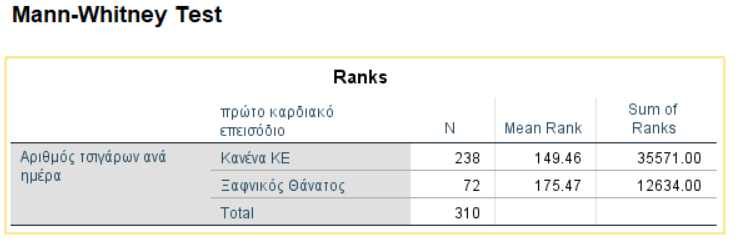
\includegraphics[width=0.8\textwidth]{images/208.PNG}
\end{figure}

\vspace{1cm}

\begin{figure}[h]
    \centering
    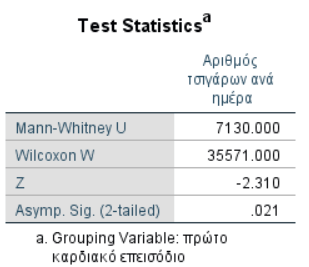
\includegraphics[width=0.4\textwidth]{images/209.PNG}
\end{figure}

Για τις διαφορές “Ακίνδυνο” και “Επικίνδυνο” φαίνεται ότι δεν υπάρχει στατιστικά σημαντική διαφορά στις μέσες τιμές σε σχέση με τον “Αριθμό τσιγάρων”. Αυτό προκύπτει από το γεγονός ότι το p-value είναι >5\%. Δηλαδή ο αριθμός τσιγάρων που καπνίζεται από τις δυο κατηγορίες είναι ίδιος.

\begin{figure}[h]
    \centering
    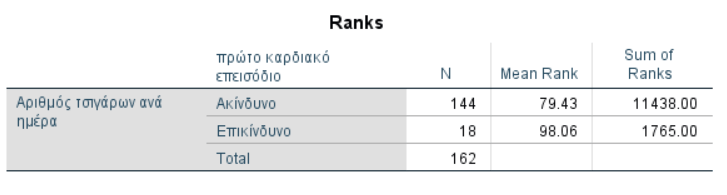
\includegraphics[width=0.8\textwidth]{images/210.PNG}
\end{figure}

\clearpage

\begin{figure}[ht]
    \centering
    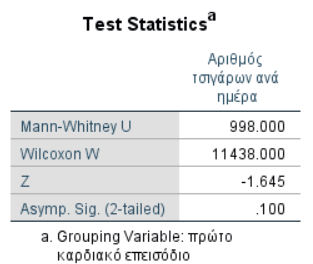
\includegraphics[width=0.4\textwidth]{images/211.PNG}
\end{figure}

Για τις διαφορές “Ακίνδυνο” και “Ξαφνικός θάνατος” φαίνεται ότι δεν υπάρχει στατιστικά σημαντική διαφορά στις μέσες τιμές σε σχέση με τον “Αριθμό τσιγάρων”. Αυτό προκύπτει από το γεγονός ότι το p-value είναι >5\%. Δηλαδή ο αριθμός τσιγάρων που καπνίζεται από τις δυο κατηγορίες είναι ίδιος.

\vspace{1cm}

\begin{figure}[h]
    \centering
    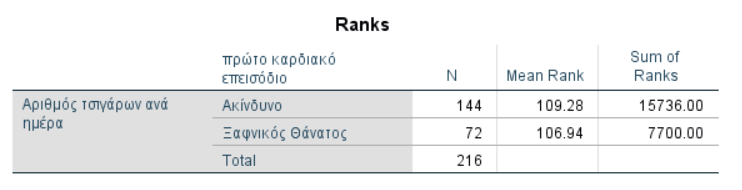
\includegraphics[width=0.8\textwidth]{images/212.PNG}
\end{figure}
\vspace{1cm}
\begin{figure}[h]
    \centering
    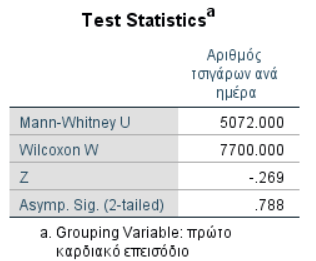
\includegraphics[width=0.4\textwidth]{images/213.PNG}
\end{figure}

\clearpage

\vspace{2cm}
Για τις διαφορές “Επικίνδυνο” και “Ξαφνικός θάνατος” φαίνεται ότι δεν υπάρχει στατιστικά σημαντική διαφορά στις μέσες τιμές σε σχέση με τον “Αριθμό τσιγάρων”. Αυτό προκύπτει από το γεγονός ότι το p-value είναι >5\%. Δηλαδή ο αριθμός τσιγάρων που καπνίζεται από τις δυο κατηγορίες είναι ίδιος.

\vspace{1cm}

\begin{figure}[h]
    \centering
    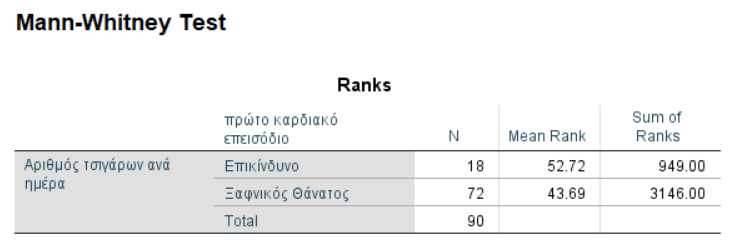
\includegraphics[width=0.8\textwidth]{images/214.PNG}
\end{figure}
\vspace{1cm}
\begin{figure}[h]
    \centering
    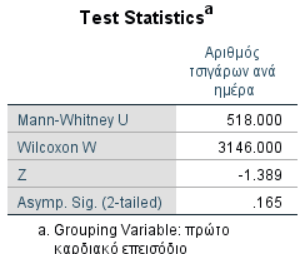
\includegraphics[width=0.4\textwidth]{images/215.PNG}
\end{figure}

\clearpage
Ο πίνακας \lat{Case Processing Summary}  μας δίνει πληροφορίες για το πόσα από τα \lat{cases} που υπήρχαν αρχικά στο αρχείο μας, λήφθηκαν υπόψιν, στην μελέτη των κατηγοριών του "Πρώτου καρδιακού επισοδείου" σε σχέση με την "Μέση διαστολική αρτηριακή πίεση".

\begin{figure}[h]
    \centering
    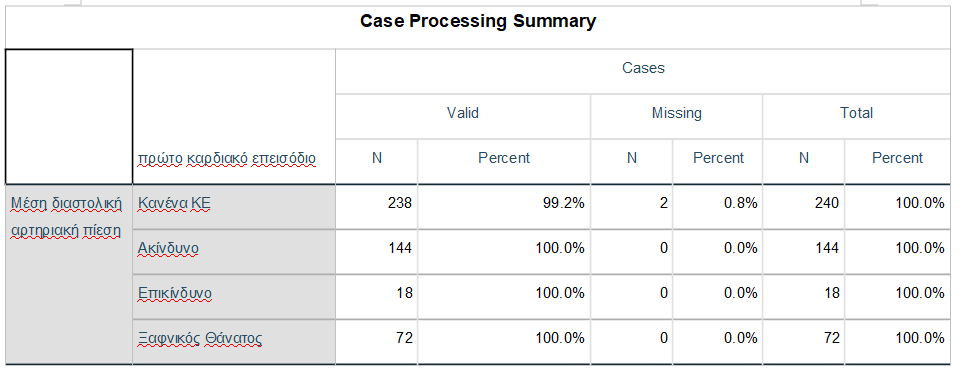
\includegraphics[width=\textwidth]{images/125.PNG}
\end{figure}
\vspace{1cm}
Από τον πίνακα \textbf{\lat{Tests of Normality}} μπορούμε να πάρουμε αποτελέσματα από δύο τεστ κανονικότητας, τα \lat{Kolmogorov-Smirnov} και \lat{Shapiro-Wilk}. Παρατηρώντας τον πίνακα βλέπουμε ότι το p-value εκτός της υποομάδας που έχει τον χαρακτηρισμό Επικίνδυνο, είναι μικρότερο του 5\%. Δηλαδή, δεν ακολουθούν κανονική κατανομή.  Λόγω αυτού, θα  χρησιμοποιήσουμε τον μη-παραμετρικό έλεγχο διαφορών ανάμεσα σε περισσότερες από δύο ανεξάρτητες ομάδες, \lat{Kruskal-Wallis H}. 
\vspace{1cm}
\begin{figure}[h]
    \centering
    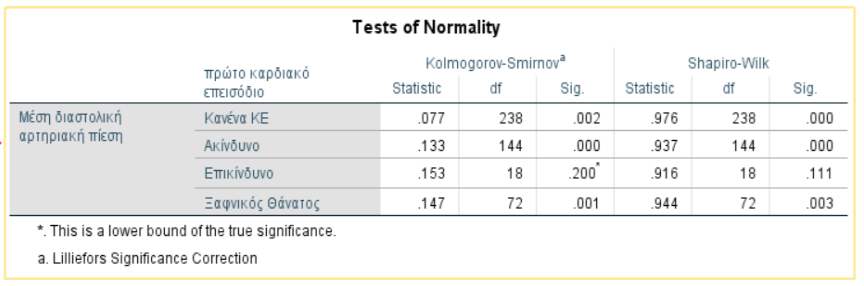
\includegraphics[width=\textwidth]{images/126.PNG}
\end{figure}

\clearpage

\begin{figure}[h]
 \centering

     \begin{subfigure}{0.8\textwidth}
     \centering
         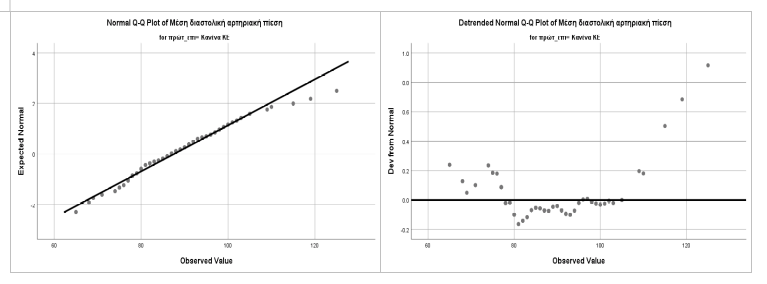
\includegraphics[width=\textwidth]{images/127.PNG}
                      \end{subfigure}
     
     \begin{subfigure}{0.8\textwidth}
     \centering
         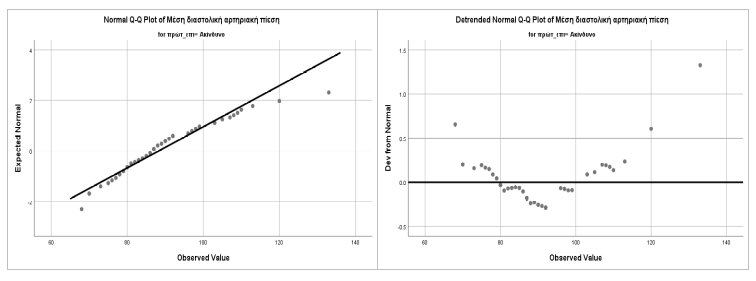
\includegraphics[width=\textwidth]{images/128.PNG}
                    \end{subfigure}
                    
                    \begin{subfigure}{0.8\textwidth}
     \centering
         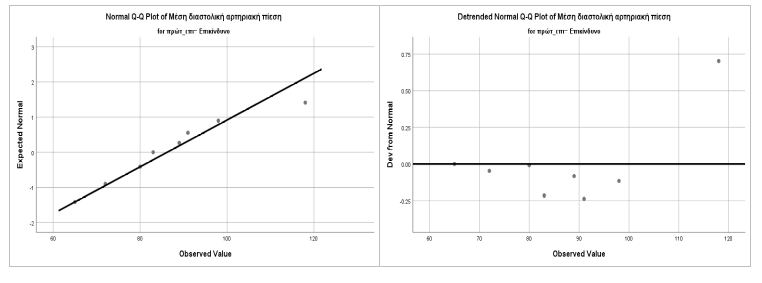
\includegraphics[width=\textwidth]{images/129.PNG}
                    \end{subfigure}
                    
                    \begin{subfigure}{0.8\textwidth}
     \centering
         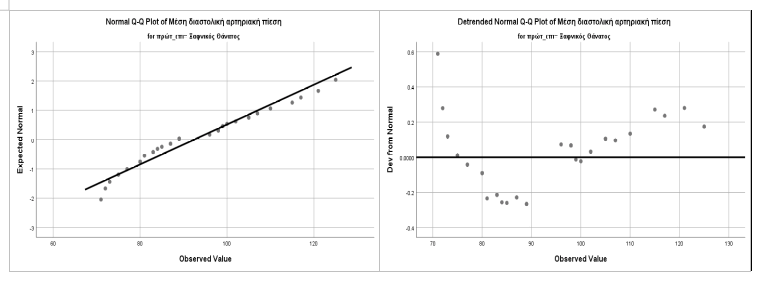
\includegraphics[width=\textwidth]{images/130.PNG}
                    \end{subfigure}
\end{figure}

\clearpage

\begin{figure}[ht]
    \centering
    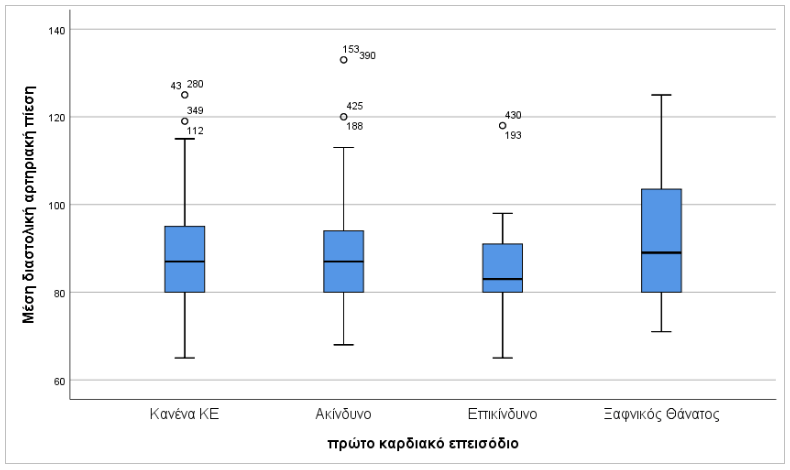
\includegraphics[width=\textwidth]{images/131.PNG}
\end{figure}

Από τον πίνακα \textbf{\lat{Test Statistics}} προκύπτει ότι  το p-value είναι >5\%. Συνεπώς δεν υπάρχουν σημαντικές διαφορές στη τιμή της  Μέσης διαστολικής αρτηριακής πίεσης σε σχέση με το πρώτο καρδιακό επεισόδιο. Άρα, η μέση διαστολική αρτηριακή πίεση φαίνεται να μην επηρεάζεται παρόλο την κατηγορία επικινδυνότητας του πρώτου καρδιακού επεισοδίου.

\begin{figure}[h]
    \centering
    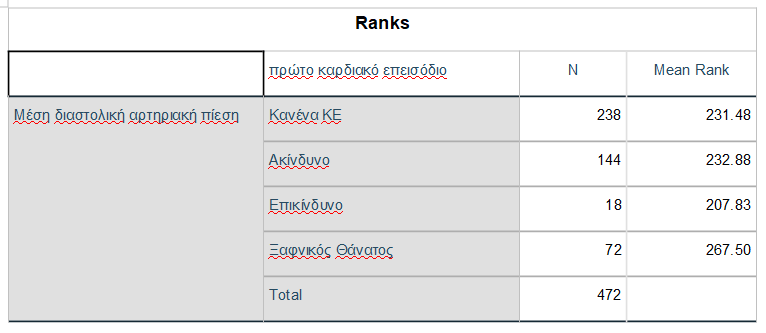
\includegraphics[width=0.8\textwidth]{images/132.PNG}
\end{figure}

\clearpage

\begin{figure}[ht]
    \centering
    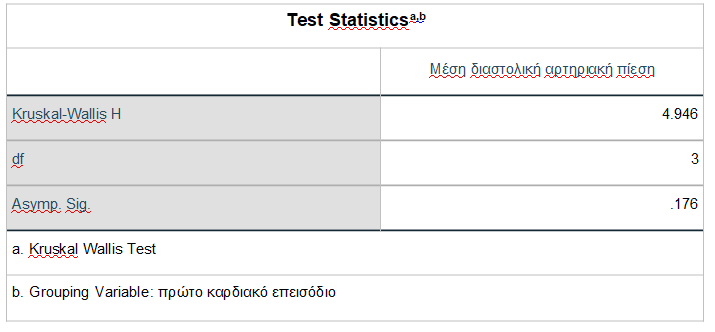
\includegraphics[width=0.6\textwidth]{images/133.PNG}
\end{figure}